\documentclass[11pt]{charter}

% El títulos de la memoria, se usa en la carátula y se puede usar el cualquier lugar del documento con el comando \ttitle
\titulo{Mantenimiento predictivo usando cómputo en la nube} 

% Nombre del posgrado, se usa en la carátula y se puede usar el cualquier lugar del documento con el comando \degreename
%\posgrado{Carrera de Especialización en Sistemas Embebidos} 
\posgrado{Carrera de Especialización en Internet de las Cosas} 
%\posgrado{Carrera de Especialización en Intelegencia Artificial}
%\posgrado{Maestría en Sistemas Embebidos} 
%\posgrado{Maestría en Internet de las cosas}

% Tu nombre, se puede usar el cualquier lugar del documento con el comando \authorname
\autor{Juan Pablo Pilorget} 

% El nombre del director y co-director, se puede usar el cualquier lugar del documento con el comando \supname y \cosupname y \pertesupname y \pertecosupname
\director{Director de Trabajo}
\pertenenciaDirector{Pertenencia institucional} 
% FIXME:NO IMPLEMENTADO EL CODIRECTOR ni su pertenencia
\codirector{} % si queda vacio no se deberíá incluir 
\pertenenciaCoDirector{}

% Nombre del cliente, quien va a aprobar los resultados del proyecto, se puede usar con el comando \clientename y \empclientename
\cliente{Ariel Lutenberg}
\empresaCliente{Carrera de Especialización en IoT - FIUBA}

% Nombre y pertenencia de los jurados, se pueden usar el cualquier lugar del documento con el comando \jurunoname, \jurdosname y \jurtresname y \perteunoname, \pertedosname y \pertetresname.
\juradoUno{Nombre y Apellido (1)}
\pertenenciaJurUno{pertenencia (1)} 
\juradoDos{Nombre y Apellido (2)}
\pertenenciaJurDos{pertenencia (2)}
\juradoTres{Nombre y Apellido (3)}
\pertenenciaJurTres{pertenencia (3)}
 
\fechaINICIO{25 de agosto de 2020}		%Fecha de inicio de la cursada de GdP \fechaInicioName
\fechaFINALPlanificacion{13 de octubre de 2020} 	%Fecha de final de cursada de GdP
\fechaFINALTrabajo{1 de julio de 2021}		%Fecha de defensa pública del trabajo final


\begin{document}

\maketitle
\thispagestyle{empty}
\pagebreak


\thispagestyle{empty}
{\setlength{\parskip}{0pt}
\tableofcontents{}
}
\pagebreak


\section{Registros de cambios}
\label{sec:registro}


\begin{table}[ht]
\label{tab:registro}
\centering
\begin{tabularx}{\linewidth}{@{}|c|X|c|@{}}
\hline
\rowcolor[HTML]{C0C0C0} 
Revisión & \multicolumn{1}{c|}{\cellcolor[HTML]{C0C0C0}Detalles de los cambios realizados} & Fecha      \\ \hline
1.0      & Creación del documento                                          & 28/08/2020 \\ \hline
1.1      &  Actualización de secciones 1 a 3                           & 04/09/2020 \\ \hline
1.2      & Actualización de secciones 4 a 6                            & 06/09/2020 \\ \hline
\end{tabularx}
\end{table}

\pagebreak



\section{Acta de constitución del proyecto}
\label{sec:acta}

\begin{flushright}
Buenos Aires, \fechaInicioName
\end{flushright}

\vspace{2cm}

Por medio de la presente se acuerda con el Ing. \authorname\hspace{1px} que su Trabajo Final de la \degreename\hspace{1px} se titulará ``\ttitle'', consistirá esencialmente en el prototipo preliminar de un sistema de control de temperatura de un calefón, y tendrá un presupuesto preliminar estimado de 600 hs de trabajo y USD 21.250, con fecha de inicio \fechaInicioName\hspace{1px} y fecha de presentación pública \fechaFinalName.

Se adjunta a esta acta la planificación inicial.

\vfill

% Esta parte se construye sola con la información que hayan cargado en el preámbulo del documento y no debe modificarla
\begin{table}[ht]
\centering
\begin{tabular}{ccc}
\begin{tabular}[c]{@{}c@{}}Ariel Lutenberg \\ Director posgrado FIUBA\end{tabular} & \hspace{2cm} & \begin{tabular}[c]{@{}c@{}}\clientename \\ \empclientename \end{tabular} \vspace{2.5cm} \\ 
\multicolumn{3}{c}{\begin{tabular}[c]{@{}c@{}} \supname \\ Director del Trabajo Final\end{tabular}} \vspace{2.5cm} \\
%\begin{tabular}[c]{@{}c@{}}\jurunoname \\ Jurado del Trabajo Final\end{tabular}     &  & \begin{tabular}[c]{@{}c@{}}\jurdosname\\ Jurado del Trabajo Final\end{tabular}  \vspace{2.5cm}  \\
%\multicolumn{3}{c}{\begin{tabular}[c]{@{}c@{}} \jurtresname\\ Jurado del Trabajo Final\end{tabular}} \vspace{.5cm}                                                                     
\end{tabular}
\end{table}




\section{Descripción técnica-conceptual del proyecto a realizar}
\label{sec:descripcion}

\begin{consigna}{black}
La integración cada vez mayor de la tecnología operacional al mundo IoT plantea desafíos y numerosas oportunidades de desarrollo. 

Una de las nuevas oportunidades es la relacionada a la mejora en la detección y prevención de mantenimiento de los equipos. Los procesos habituales de detección de fallas están vinculados a fallas concretas en el equipamiento o a controles de rutina, con un esfuerzo operacional y un costo económico elevado. Al incorporar capacidades de analítica avanzada no sólo se vuelve más efectivo el proceso -reduciendo los tiempos muertos generados por los controles de rutina- sino que además disminuye el deterioro de los equipos al realizar el mantenimiento de forma preventiva. 

A la vez, la capacidad de ejecutar tareas intensivas de cómputo en la nube permiten escalar los recursos de manera elástica, es decir, aprovisionando recursos para las tareas específicas en cada momento, y escalable, esto es, permitiendo ir conectando dispositivos sin estar limitados por la infraestructura de cómputo subyacente.

En la figura 1 se observa la arquitectura de referencia para solucionar el problema propuesto.


\vspace{25px}

\begin{figure}[htpb]
\centering 
\includegraphics[width=.8\textwidth]{./Figuras/diagrama-bloques.png}
\caption{Diagrama en bloques del sistema}
\label{fig:diagBloques}
\end{figure}


\vspace{25px}

El objetivo de la arquitectura propuesta es identificar anomalías en las señales -si nuestro dispositivo de origen es una turbina de viento, un ejemplo de señales pueden ser la velocidad del rotor, la velocidad del viento o la temperatura exterior- emitidas por los controladores lógicos programables (PLC, por su acrónimo en inglés). Para ello, se pretende desarrollar una arquitectura que, en primer lugar, tome la información de los PLC mediante la tecnología de comunicación industrial OPC-UA y la transmita de manera segura. La arquitectura también debe permitir operar fuera de línea, sincronizando con la nube al recuperar la conectividad. Para este punto se pretende usar AWS IoT Greengrass. En caso de querer modelar también la conexión de los PLC y simular información proveniente de, por ejemplo, turbinas de viento, se puede utilizar la versión demo de KepServerEX. 

Posteriormente, se busca modelar los activos y poder monitorearlos para, mediante reglas, realizar procesos analíticos con esa información. El proceso de modelado y estructuración se diseñó utilizando AWS IoT SiteWise y AWS IoT Core y la analítica se desea calcular con AWS IoT Analytics. 

En este punto es donde se dispara el proceso de detección de anomalías. En primer lugar, un modelo de aprendizaje automático -potencialmente uno de tipo Isolation Forest- entrenado en Amazon SageMaker se disponibiliza (mediante containers) y realiza la inferencia para la información estructurada que ingresa desde AWS IoT Analytics. En segundo lugar, se crea una notificación mediante AWS IoT Events si se cumple una determinada regla, por ejemplo, que un conjunto de predicciones esté consistentemente por encima de un umbral específico. Finalmente, la información producida se puede visualizar de manera periódica mediante un tablero de Amazon Quicksight.

\end{consigna}


\section{Identificación y análisis de los interesados}
\label{sec:interesados}

\begin{consigna}{red} 
\begin{table}[ht]
%\caption{Identificación de los interesados}
%\label{tab:interesados}
\begin{tabularx}{\linewidth}{@{}|l|X|X|l|@{}}
\hline
\rowcolor[HTML]{C0C0C0} 
Rol           & Nombre y Apellido & Organización 	& Puesto 	\\ \hline
Auspiciante   &  \authorname                 &        FIUBA      	&  Alumno      	\\ \hline
Cliente       & \clientename      &\empclientename	&     Director 	\\ \hline
Impulsor      &  -                 &         -     	&     -	\\ \hline
Responsable   & \authorname       & FIUBA        	& Alumno 	\\ \hline
Colaboradores & Consultor experto en IoT                  &    Amazon Web Services   	& IoT Subject Matter Expert       	\\ \hline
Orientador    & \supname	      & \pertesupname 	& Director	Trabajo final \\ \hline
Usuario final &   -             &     Empresa        	&        Ingeniero de procesos / operaciones \\ \hline
\end{tabularx}
\end{table}

\end{consigna}



\section{1. Propósito del proyecto}
\label{sec:proposito}

\begin{consigna}{black}
El propósito de este proyecto es mejorar los actuales procesos de detección de necesidad de mantenimiento en equipamiento industrial, reduciendo tiempos y costos e incrementando la productividad. Para ello, se pretende desarrollar un flujo de trabajo que integre de manera completa -punta a punta- desde la captación de eventos en el dispositivo de borde hasta la inferencia mediante aprendizaje automático.
\end{consigna}

\section{2. Alcance del proyecto}
\label{sec:alcance}

\begin{consigna}{black}
El alcance del proyecto contempla el desarrollo de la arquitectura de transmisión de la información desde los PLC hacia la nube, su análisis y visualización para la detección temprana de necesidad de mantenimiento. 

El presente proyecto no incluye la conexión en un ámbito industrial del equipamiento. Dicho flujo se simulará utilizando herramientas como KepServerEX.

\end{consigna}


\section{3. Supuestos del proyecto}
\label{sec:supuestos}

\begin{consigna}{black}
Para el desarrollo del presente proyecto se supone que:

\begin{itemize}
\item Se cuenta con acceso a servicios de cómputo en la nube (en este caso, Amazon Web Services).
\item La simulación de PLC mediante \textit{software} es condición suficiente para demostrar la viabilidad técnica y financiera del proyecto.
\item Se contará con información de dominio suficiente del ámbito industrial a elegir.
\end{itemize}

\end{consigna}

\section{4. Requerimientos}
\label{sec:requerimientos}
\begin{consigna}{black}
\begin{enumerate}
\item Grupo de requerimientos asociados con \textit{hardware}:
	\begin{enumerate}
	\item Debe enviar señales simulando un PLC mediante un dispositivo de tipo Raspberry Pi.
	\item Debe usar un protocolo de tipo OPC-UA.
	\item Debe recolectar y procesar la información en la nube.
	\item Debe realizar inferencias y permitir visualizarlas en la nube.
	\item Debe almacenar la información de los PLC en la nube.
	\end{enumerate}
\item Grupo de requerimientos asociados con \textit{software}:
	\begin{enumerate}
	\item Debe dirigir la información recibida desde los PLC y redirigida a la nube mediante un motor de reglas.
	\item Debe incluir un modelo de aprendizaje automático de detección de anomalías.
	\item Debe presentar los resultados del modelo de aprendizaje automático detectados como anómalos en \textit{near real-time} mediante un tablero.
	\item Debe generar notificaciones (a ser enviadas a un correo electrónico o mediante SMS).
	\end{enumerate}
\end{enumerate}

\end{consigna}

\section{Historias de usuarios (\textit{Product backlog})}
\label{sec:backlog}
\begin{consigna}{black}
\begin{itemize}
\item Como líder técnico del proyecto quiero construir un listado exhaustivo de épicas, historias de usuario, tareas y su respectivo sprint plan. \textit{Story points: 1}
\item Como arquitecto de datos quiero desarrollar un diseño detallado de la arquitectura a construir para cumplir con los requerimientos del proyecto. \textit{Story points: 3}
\item Como arquitecto de infraestructura quiero construir un vínculo con la red corporativa mediante protocolos estándar para comunicarme con la planta y obtener los datos de los dispositivos existentes. \textit{Story points: 7}
\item Como arquitecto de datos quiero construir una flujo de procesamiento para la ingestión, almacenamiento y procesamiento de datos en tiempo real. \textit{Story points: 10}
\item Como ingeniero de operaciones quiero ser capaz de monitorear en tiempo real los indicadores operacionales clave mediante un tablero. \textit{Story points: 3}
\item Como ingeniero de operaciones quiero monitorear y gestionar las alarmas, alertas y notificaciones para las acciones. \textit{Story points: 1}
\item Como científico de datos quiero construir, entrenar y poner en producción los modelos de analítica avanzada para eficiencia operacional utilizando cómputo en la nube. \textit{Story points: 7}
\item Como líder técnico quiero tener la capacidad de automatizar el proceso de construcción de infraestructura mediante código para reducir los tiempos de despliegue. \textit{Story points: 3}
\end{itemize}

%Descripción: En esta sección se deben incluir las historias de usuarios y su ponderación (\textit{story points}). Recordar que las historias de usuarios son descripciones cortas y simples de una característica contada desde la perspectiva de la persona que desea la nueva capacidad, generalmente un usuario o cliente del sistema. La ponderación es un número entero que representa el tamaño de la historia comparada con otras historias de similar tipo.
\end{consigna}

\section{5. Entregables principales del proyecto}
\label{sec:entregables}

\begin{consigna}{black}
Los entregables principales del proyecto serán: 
\begin{itemize}
\item Documentación describiendo el paso a paso de despliegue de la solución y los artefactos asociados (\textit{runbook})
\item Documentación detallando los pasos para la operación de la solución (\textit{playbook})
\item Artefactos de infraestructura como código para la construcción de la arquitectura
\item Código fuente de los modelos de aprendizaje automático desarrollados
\item Informe final de presentación de resultados

\end{itemize}

\end{consigna}

\section{6. Desglose del trabajo en tareas}
\label{sec:wbs}
Todas las tareas se estiman en múltiplos de días completos (jornadas de 8 horas) para llegar al siguiente conjunto de tareas:
\begin{consigna}{black}
\begin{enumerate}

\item \textbf{Planificación del proyecto (48 hs)}
	\begin{enumerate}
	\item Definición del plan de proyecto (24 hs)
	\item Desglose de tareas del plan  (16 hs)
	\item Aprobación del plan (8 hs)
	\end{enumerate}

\item \textbf{Investigación preliminar (72 hs)}
	\begin{enumerate}
	\item Análisis de casos de uso similares (16 hs)
	\item Revisión de documentación de servicios propuestos (32 hs)
	\item Evaluación de alternativas de simulación de datos (16 hs)
	\item Recopilación de código y documentación de soluciones (8 hs)
	\end{enumerate}

\item \textbf{Prueba de concepto (112 hs)}
	\begin{enumerate}
	\item Creación de cuentas y definición de permisos (16 hs)
	\item Compra de equipamiento (8 hs)
	\item Desarrollo de arquitectura (40 hs)
	\item Construcción de \textit{wireframe} (40 hs)
	\item Evaluación de funcionamiento (8 hs)
	\end{enumerate}
	
\item \textbf{Implementación (168 hs)}
	\begin{enumerate}
	\item Creación de representación virtual de datos validados (40 hs)
	\item Recolección e ingesta en la nube de los datos (32hs)
	\item Definición de monitoreo de parámetros (8 hs)
	\item Desarrollo de modelo de analítica avanzada (32hs)
	\item Construccion de tablero de control (24 hs)
	\item Confección de notificaciones y alertas (16 hs)
	\item Creación de plantilla de infraestructura como código (16 hs)
	\end{enumerate}

\item \textbf{Validación (72 hs)}
	\begin{enumerate}
	\item Evaluación de desempeño con datos en tiempo real (32hs)
	\item Realización de pruebas UAT para interfaz (24 hs)
	\item Evaluación de desempeño de alertas y notificaciones (16 hs)
	\end{enumerate}

\item \textbf{Documentación y presentación (128 hs)}
	\begin{enumerate}
	\item Confección de la memoria (40 hs)
	\item Confección del \textit{playbook} (32 hs)
	\item Confección del \textit{runbook} (32 hs)
	\item Desarrollo de la presentación (16 hs)
	\item Presentación (8 hs)
	\end{enumerate}
\end{enumerate}

Cantidad total de horas: 600 hs

\end{consigna}

\section{7. Diagrama de Activity On Node}
\label{sec:AoN}
\begin{consigna}{black}
%La figura \ref{fig:AoN} fue elaborada con el paquete latex tikz y pueden consultar la siguiente referencia \textit{online}:

%\url{https://www.overleaf.com/learn/latex/LaTeX_Graphics_using_TikZ:_A_Tutorial_for_Beginners_(Part_3)\%E2\%80\%94Creating_Flowcharts}
A continuación se presenta el diagrama de \textit{Activity on Node} para el proyecto, coloreado según los grupos de tareas definidas en el apartado inmediato anterior. 
\end{consigna}

\begin{figure}[htpb]
\centering 
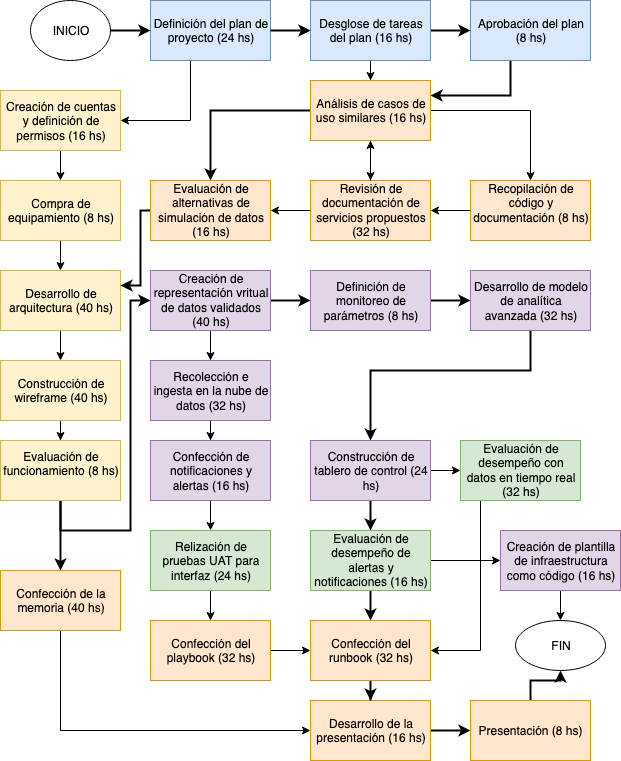
\includegraphics[width=.9\textwidth]{./Figuras/AoN.png}
\caption{Diagrama \textit{Activity on Node}}
\label{fig:AON}
\end{figure}


\section{8. Diagrama de Gantt}
\label{sec:gantt}
A continuación se presenta el diagrama de Gantt con las fechas preliminares a revisar y alinear a la fecha de cierre y presentación definida en el acta constitutiva.

\begin{figure}[htpb]
\centering 
\includegraphics[width=1\textwidth]{./Figuras/gantt.png}
\caption{Diagrama de Gantt}
\label{fig:Gantt}
\end{figure}


\section{9. Matriz de uso de recursos de materiales}
\label{sec:recursos}
Para cada tarea desagregada se asigna una estimación de recusos -en horas- y se las agrupa según código de WBS (grupos de tareas según propósito), como se detalla en la siguiente tabla. 
\begin{table}
\label{tab:recursos}
\centering
\begin{tabularx}{\linewidth}{@{}|c|c|c|c|c|@{}}
\hline
\cellcolor[HTML]{C0C0C0} & \cellcolor[HTML]{C0C0C0} & \multicolumn{3}{c|}{\cellcolor[HTML]{C0C0C0}Recursos (hs)} \\ \cline{3-5} 
\multirow{-2}{*}{\cellcolor[HTML]{C0C0C0}\begin{tabular}[c]{@{}c@{}}Código\\ WBS\end{tabular}} & \multirow{-2}{*}{\cellcolor[HTML]{C0C0C0}\begin{tabular}[c]{@{}c@{}}Nombre \\ tarea\end{tabular}} & PC & HW & Rev\\ \hline
Planificación del proyecto & Definición del plan de proyecto & 24 &  &  \\ \hline
Planificación del proyecto & Desglose de tareas del plan &  &  & 16  \\ \hline
Planificación del proyecto & Aprobación del plan &  &  & 8 \\ \hline
Investigación preliminar & Análisis de casos de uso similares 16 &  &  &  \\ \hline
Investigación preliminar & Evaluación de alternativas de simulación & 16  &  &  \\ \hline
Investigación preliminar & Revisión de documentación de servicios &  32 &  &  \\ \hline
Investigación preliminar & Recopilación de código y documentación & 8 &  &  \\ \hline
Prueba de concepto & Creación de cuentas y definición de permisos & 16 &  &  \\ \hline 
Prueba de concepto & Compra de equipamiento &  & 8 &  \\ \hline
Prueba de concepto & Desarrollo de arquitectura & 20 & 20 &  \\ \hline
Prueba de concepto & Construcción de \textit{wireframe} & 30 & 10 &  \\ \hline
Prueba de concepto & Evaluación de funcionamiento &  &  & 8 \\ \hline
Implementación & Creación de representación virtual de datos &  20 & 20 &  \\ \hline
Implementación & Recolección de datos e ingesta en la nube & 24 & 8  &  \\ \hline
Implementación & Definición de monitoreo de parámetros & 8 &  &  \\ \hline
Implementación & Desarrollo de modelo de analítica avanzada & 32 &  &  \\ \hline
Implementación & Construcción de tablero de control & 24 &  &  \\ \hline
Implementación & Confección de notificaciones y alertas & 16 &  &  \\ \hline
Implementación & Creación de plantilla de IaC &  & 16 &  \\ \hline
Validación & Evaluación de desempeño en tiempo real & 32 &  &  \\ \hline
Validación & Realización de pruebas UAT para interfaz & 24 &  &  \\ \hline
Validación & Evaluación de desempeño de alertas & 16 &  &  \\ \hline
Documentación y pres. & Confección de la memoria & 32 &  & 8 \\ \hline
Documentación y pres.& Confección del playbook & 32 &  &  \\ \hline 
Documentación y pres.& Confección del runbook & 32 &  &  \\ \hline
Documentación y pres.& Desarrollo de la presentación & 8 &  & 8  \\ \hline
Documentación y pres.& Presentación & 4 &  & 4 \\ \hline
\end{tabularx}%
\end{table}

{\footnotesize
Referencias:
\begin{itemize}
	\item PC = Investigación, redacción y desarrollo de software
	\item HW = Compra y desarrollo de hardware
	\item Rev = Revisión de terceros
\end{itemize}
} %footnotesize


\section{10. Presupuesto detallado del proyecto}
\label{sec:presupuesto}

\begin{consigna}{black}

\begin{table}[htpb]
\centering
\begin{tabularx}{\linewidth}{@{}|X|c|r|r|@{}}
\hline
\rowcolor[HTML]{C0C0C0} 
\multicolumn{4}{|c|}{\cellcolor[HTML]{C0C0C0}COSTOS DIRECTOS} \\ \hline
\rowcolor[HTML]{C0C0C0} 
Descripción &
  \multicolumn{1}{c|}{\cellcolor[HTML]{C0C0C0}Cantidad} &
  \multicolumn{1}{c|}{\cellcolor[HTML]{C0C0C0}Valor unitario} &
  \multicolumn{1}{c|}{\cellcolor[HTML]{C0C0C0}Valor total} \\ \hline
Horas de desarrollo & 
  \multicolumn{1}{c|}{600} & 
  \multicolumn{1}{c|}{25} & 
  \multicolumn{1}{c|}{15000} \\ \hline
Horas de cómputo en la nube &
  \multicolumn{1}{c|}{1200} & 
  \multicolumn{1}{c|}{1,5} & 
  \multicolumn{1}{c|}{1800} \\ \hline
  Raspberry Pi y periféricos & 
  \multicolumn{1}{c|}{1} & 
  \multicolumn{1}{c|}{150} & 
  \multicolumn{1}{c|}{150} \\ \hline
Materiales varios &
  \multicolumn{1}{c|}{1} & 
  \multicolumn{1}{c|}{50} & 
  \multicolumn{1}{c|}{50} \\ \hline

\multicolumn{3}{|c|}{SUBTOTAL} &
  \multicolumn{1}{c|}{} \\ \hline
\rowcolor[HTML]{C0C0C0} 
\multicolumn{4}{|c|}{\cellcolor[HTML]{C0C0C0}COSTOS INDIRECTOS} \\ \hline
\rowcolor[HTML]{C0C0C0} 
Descripción &
  \multicolumn{1}{c|}{\cellcolor[HTML]{C0C0C0}Cantidad} &
  \multicolumn{1}{c|}{\cellcolor[HTML]{C0C0C0}Valor unitario} &
  \multicolumn{1}{c|}{\cellcolor[HTML]{C0C0C0}Valor total} \\ \hline
\multicolumn{1}{|l|}{25\% del costo directo (hs de revisión de terceros)} &
   1 & 
   4250 &
  4250  \\ \hline
\multicolumn{1}{|l|}{} &
   &
   &
   \\ \hline
\multicolumn{3}{|c|}{SUBTOTAL} &
  \multicolumn{1}{c|}{21250} \\ \hline
\rowcolor[HTML]{C0C0C0}
\multicolumn{3}{|c|}{TOTAL} &
 21250  \\ \hline
\end{tabularx}%
\end{table}

\end{consigna}

\section{11. Matriz de asignación de responsabilidades}
\label{sec:responsabilidades}
\begin{consigna}{black}
La asignación de responsabilidades y el manejo de la autoridad del proyecto se gestionará de la siguiente manera:

\begin{table}[htpb]
\centering
\resizebox{\textwidth}{!}{%
\begin{tabular}{|c|c|c|c|c|c|}
\hline
\rowcolor[HTML]{C0C0C0} 
\cellcolor[HTML]{C0C0C0} &
  \cellcolor[HTML]{C0C0C0} &
  \multicolumn{4}{c|}{\cellcolor[HTML]{C0C0C0}Nombres y roles del proyecto} \\ \cline{3-6} 
\rowcolor[HTML]{C0C0C0} 
\cellcolor[HTML]{C0C0C0} &
  \cellcolor[HTML]{C0C0C0} &
  Responsable &
  Orientador &
  Equipo &
  Cliente \\ \cline{3-6} 
\rowcolor[HTML]{C0C0C0} 
\multirow{-3}{*}{\cellcolor[HTML]{C0C0C0}\begin{tabular}[c]{@{}c@{}}Código\\ WBS\end{tabular}} &
  \multirow{-3}{*}{\cellcolor[HTML]{C0C0C0}Nombre de la tarea} &
  \authorname &
  \supname &
  Experto en IoT &
  \clientename \\ \hline
Planificación del proyecto & Definición del plan de proyecto & P & A & & C \\ \hline
Planificación del proyecto & Desglose de tareas del plan & P & I &  & I  \\ \hline
Planificación del proyecto & Aprobación del plan & P & A & & I \\ \hline
Investigación preliminar & Análisis de casos de uso similares & P & I  & C &  \\ \hline
Investigación preliminar & Evaluación de alternativas de simulación & P  &  & C & I \\ \hline
Investigación preliminar & Revisión de documentación de servicios &  P &  & I &  \\ \hline
Investigación preliminar & Recopilación de código y documentación & P & & C &  \\ \hline
Prueba de concepto & Creación de cuentas y definición de permisos & P & & & I \\ \hline 
Prueba de concepto & Compra de equipamiento & P & & C &  \\ \hline
Prueba de concepto & Desarrollo de arquitectura & P & A & C &  \\ \hline
Prueba de concepto & Construcción de \textit{wireframe} & P & A &  & A  \\ \hline
Prueba de concepto & Evaluación de funcionamiento & P & I &  & I \\ \hline
Implementación & Creación de representación virtual de datos &  P & & C &  \\ \hline
Implementación & Recolección de datos e ingesta en la nube & P &  &  &  \\ \hline
Implementación & Definición de monitoreo de parámetros & P &  & & C  \\ \hline
Implementación & Desarrollo de modelo de analítica avanzada & P &  & C & A  \\ \hline
Implementación & Construcción de tablero de control & P & & C & A \\ \hline
Implementación & Confección de notificaciones y alertas & P & &  & A \\ \hline
Implementación & Creación de plantilla de IaC & P & & C & I \\ \hline
Validación & Evaluación de desempeño en tiempo real & P & I & & A \\ \hline
Validación & Realización de pruebas UAT para interfaz & P & I & & A \\ \hline
Validación & Evaluación de desempeño de alertas & P & I &  & A \\ \hline
Documentación y pres. & Confección de la memoria & P & A &  &  \\ \hline
Documentación y pres.& Confección del playbook & P & I &  & A \\ \hline 
Documentación y pres.& Confección del runbook & P & I & & A \\ \hline
Documentación y pres.& Desarrollo de la presentación & P & A & &  \\ \hline
Documentación y pres.& Presentación & P & A &  & \\ \hline
\end{tabular}%
}
\end{table}


{\footnotesize
Referencias:
\begin{itemize}
	\item P = Responsabilidad Primaria
	\item S = Responsabilidad Secundaria
	\item A = Aprobación
	\item I = Informado
	\item C = Consultado
\end{itemize}
} %footnotesize

%Una de las columnas debe ser para el Director, ya que se supone que participará en el proyecto.
%A su vez se debe cuidar que no queden muchas tareas seguidas sin ``A'' o ``I''.

\end{consigna}

\section{12. Gestión de riesgos}
\label{sec:riesgos}

\begin{consigna}{red}
a) Identificación de los riesgos (al menos cinco) y estimación de sus consecuencias:
 
Riesgo 1: detallar el riesgo (riesgo es algo que si ocurre altera los planes previstos)
\begin{itemize}
\item Severidad (S): mientras más severo, más alto es el número (usar números del 1 al 10).\\
Justificar el motivo por el cual se asigna determinado número de severidad (S).
\item Probabilidad de ocurrencia (O): mientras más probable, más alto es el número (usar del 1 al 10).\\
Justificar el motivo por el cual se asigna determinado número de (O). 
\end{itemize}   

Riesgo 2:
\begin{itemize}
\item Severidad (S): 
\item Ocurrencia (O):
\end{itemize}

Riesgo 3:
\begin{itemize}
\item Severidad (S): 
\item Ocurrencia (O):
\end{itemize}


b) Tabla de gestión de riesgos:      (El RPN se calcula como RPN=SxO)

\begin{table}[htpb]
\centering
\begin{tabularx}{\linewidth}{@{}|X|c|c|c|c|c|c|@{}}
\hline
\rowcolor[HTML]{C0C0C0} 
Riesgo & S & O & RPN & S* & O* & RPN* \\ \hline
       &   &   &     &    &    &      \\ \hline
       &   &   &     &    &    &      \\ \hline
       &   &   &     &    &    &      \\ \hline
       &   &   &     &    &    &      \\ \hline
       &   &   &     &    &    &      \\ \hline
\end{tabularx}%
\end{table}

Criterio adoptado: 
Se tomarán medidas de mitigación en los riesgos cuyos números de RPN sean mayores a...

Nota: los valores marcados con (*) en la tabla corresponden luego de haber aplicado la mitigación.

c) Plan de mitigación de los riesgos que originalmente excedían el RPN máximo establecido:
 
Riesgo 1: plan de mitigación (si por el RPN fuera necesario elaborar un plan de mitigación).
  Nueva asignación de S y O, con su respectiva justificación:
  - Severidad (S): mientras más severo, más alto es el número (usar números del 1 al 10).
          Justificar el motivo por el cual se asigna determinado número de severidad (S).
  - Probabilidad de ocurrencia (O): mientras más probable, más alto es el número (usar del 1 al 10).
          Justificar el motivo por el cual se asigna determinado número de (O).

Riesgo 2: plan de mitigación (si por el RPN fuera necesario elaborar un plan de mitigación).
 
Riesgo 3: plan de mitigación (si por el RPN fuera necesario elaborar un plan de mitigación).

\end{consigna}


\section{13. Gestión de la calidad}
\label{sec:calidad}

\begin{consigna}{red}
Para cada uno de los requerimientos del proyecto indique:
\begin{itemize} 
\item Req \#1: copiar acá el requerimiento.

Verificación y validación:

\begin{itemize}
\item Verificación para confirmar si se cumplió con lo requerido antes de mostrar el sistema al cliente. Detallar 
\item Validación con el cliente para confirmar que está de acuerdo en que se cumplió con lo requerido. Detallar  
\end{itemize}

\end{itemize}

Tener en cuenta que en este contexto se pueden mencionar simulaciones, cálculos, revisión de hojas de datos, consulta con expertos, mediciones, etc.

\end{consigna}

\section{14. Comunicación del proyecto}
\label{sec:comunicaciones}

El plan de comunicación del proyecto es el siguiente:

\begin{table}[htpb]
\centering
\begin{tabularx}{\linewidth}{@{}|X|C{2.4cm}|C{3cm}|C{1.8cm}|C{2cm}|C{2.1cm}|@{}}
\hline
\rowcolor[HTML]{C0C0C0} 
\multicolumn{6}{|c|}{\cellcolor[HTML]{C0C0C0}PLAN DE COMUNICACIÓN DEL PROYECTO}           \\ \hline
\rowcolor[HTML]{C0C0C0} 
¿Qué comunicar? & Audiencia & Propósito & Frecuencia & Método de comunicac. & Responsable \\ \hline
                &           &           &            &                      &             \\ \hline
                &           &           &            &                      &             \\ \hline
                &           &           &            &                      &             \\ \hline
                &           &           &            &                      &             \\ \hline
                &           &           &            &                      &             \\ \hline
\end{tabularx}
\end{table}

\section{15. Gestión de compras}
\label{sec:compras}

\begin{consigna}{red}
En caso de tener que comprar elementos o contratar servicios:
a) Explique con qué criterios elegiría a un proveedor.
b) Redacte el Statement of Work correspondiente.
\end{consigna}

\section{16. Seguimiento y control}
\label{sec:seguimiento}

\begin{consigna}{red}
Para cada tarea del proyecto establecer la frecuencia y los indicadores con los se seguirá su avance y quién será el responsable de hacer dicho seguimiento y a quién debe comunicarse la situación (en concordancia con el Plan de Comunicación del proyecto).

El indicador de avance tiene que ser algo medible, mejor incluso si se puede medir en \% de avance. Por ejemplo,se pueden indicar en esta columna cosas como ``cantidad de conexiones ruteadeas'' o ``cantidad de funciones implementadas'', pero no algo genérico y ambiguo como ``\%'', porque el lector no sabe porcentaje de qué cosa.

\end{consigna}

\begin{longtable}{|m{1cm}|m{3.5cm}|m{2.2cm}|m{2cm}|m{3cm}|m{1.5cm}|}
\hline
\rowcolor[HTML]{C0C0C0} 
\multicolumn{6}{|c|}{\cellcolor[HTML]{C0C0C0}SEGUIMIENTO DE AVANCE}                                                                       \\ \hline
\rowcolor[HTML]{C0C0C0} 
Tarea del WBS 			& Indicador de avance & Frecuencia de reporte & Resp. de seguimiento & Persona a ser informada & Método de comunic. \\ \hline
\endfirsthead

\hline
\rowcolor[HTML]{C0C0C0} 
\multicolumn{6}{c}{\cellcolor[HTML]{C0C0C0}SEGUIMIENTO DE AVANCE}                                                                       \\ \hline
\rowcolor[HTML]{C0C0C0} 
Tarea del WBS 			& Indicador de avance & Frecuencia de reporte & Resp. de seguimiento & Persona a ser informada & Método de comunic. \\ \hline
\endhead

\multicolumn{6}{c}{Continúa}
\endfoot

\endlastfoot

1.1	& Fecha de inicio  & Única vez al comienzo & \authorname & \clientename, \supname & email \\ \hline
2.1	& Avance de las subtareas  & Mensual mientras dure la tarea & \authorname & \clientename, \supname & email \\ \hline

\end{longtable}

\begin{table}[!htpb]
\centering
%\begin{tabularx}{\linewidth}{@{}|X|X|X|X|X|X|@{}}
\begin{tabularx}{\linewidth}{@{}|X|C{2.5cm}|C{3cm}|C{2cm}|C{2cm}|C{2.5cm}|@{}}
\hline
\rowcolor[HTML]{C0C0C0} 
\multicolumn{6}{|c|}{\cellcolor[HTML]{C0C0C0}SEGUIMIENTO DE AVANCE}                                                                       \\ \hline
\rowcolor[HTML]{C0C0C0} 
Tarea del WBS & Indicador de avance & Frecuencia de reporte & Resp. de seguimiento & Persona a ser informada & Método de comunic. \\ \hline
 &  &  &  &  &  \\ \hline
 &  &  &  &  &  \\ \hline
 &  &  &  &  &  \\ \hline
 &  &  &  &  &  \\ \hline
 &  &  &  &  &  \\ \hline
\end{tabularx}%
%}
\end{table}

\section{17. Procesos de cierre}    
\label{sec:cierre}

\begin{consigna}{red}
Establecer las pautas de trabajo para realizar una reunión final de evaluación del proyecto, tal que contemple las siguientes actividades:

\begin{itemize}
\item Pautas de trabajo que se seguirán para analizar si se respetó el Plan de Proyecto original:
 - Indicar quién se ocupará de hacer esto y cuál será el procedimiento a aplicar. 
\item Identificación de las técnicas y procedimientos útiles e inútiles que se utilizaron, y los problemas que surgieron y cómo se solucionaron:
 - Indicar quién se ocupará de hacer esto y cuál será el procedimiento para dejar registro.
\item Indicar quién organizará el acto de agradecimiento a todos los interesados, y en especial al equipo de trabajo y colaboradores:
  - Indicar esto y quién financiará los gastos correspondientes.
\end{itemize}

\end{consigna}


\end{document}
